% Relatório Final PIBIC-ITA
% Template baseado nas instruções oficiais do ITA
\documentclass[12pt,a4paper]{article}

% Pacotes necessários
\usepackage{iftex}
\ifPDFTeX
\usepackage[utf8]{inputenc}
\fi
\usepackage[portuguese]{babel}
\babelhyphenation{ad-vances}
\babelhyphenation{laurent varoquaux}
\ifPDFTeX
\usepackage[T1]{fontenc}
\fi
\usepackage{geometry}
\usepackage{setspace}
\usepackage{graphicx}
\usepackage{float}
\usepackage{caption}
\usepackage{subcaption}
\captionsetup[sub]{font=normalsize}
\usepackage{tabularx}
\usepackage{booktabs}
\usepackage{multirow}
\usepackage{array}
\usepackage{amsmath}
\usepackage{amsfonts}
\usepackage{amssymb}
\usepackage{fancyhdr}
\usepackage{titlesec}
\usepackage{tocloft}
\usepackage{url}
\usepackage{siunitx}
\usepackage{tikz}
\usepackage{hyperref}
\usepackage[alf]{abntex2cite}

% Configuração da página
\geometry{
    top=2cm,
    bottom=2cm,
    left=2cm,
    right=2cm
}

% Fonte: Arial (Helvetica) 12
\ifPDFTeX
\usepackage{newtxtext,newtxmath}
\else
\usepackage[no-math]{fontspec}
\setsansfont{texgyreheros}[Extension=.otf, UprightFont=*-regular, BoldFont=*-bold, ItalicFont=*-italic, BoldItalicFont=*-bolditalic]
\renewcommand{\rmdefault}{minntx}
\usepackage{newtxmath}
\setmainfont{texgyreheros}[Extension=.otf, UprightFont=*-regular, BoldFont=*-bold, ItalicFont=*-italic, BoldItalicFont=*-bolditalic]
\fi
\renewcommand{\familydefault}{\sfdefault}

% Unidades no padrão brasileiro
\sisetup{
    output-decimal-marker = {,},
    per-mode              = symbol,
    mode                  = match,
    reset-text-family     = false,
    list-final-separator  = {\ \text{e}\ },
    list-pair-separator   = {\ \text{e}\ },
    range-phrase          = {\ \text{a}\ }
}
\DeclareSIUnit{\pe}{p.e.}

% Espaçamento 1,5
\onehalfspacing
\widowpenalty=10000

% Configuração do hyperref
\hypersetup{
    colorlinks=true,
    linkcolor=black,
    filecolor=magenta,
    urlcolor=blue,
    citecolor=black
}

% Configuração dos títulos das seções
\titleformat{\section}{\normalfont\large\bfseries}{\thesection}{1em}{}
\titleformat{\subsection}{\normalfont\normalsize\bfseries}{\thesubsection}{1em}{}

% Configuração do cabeçalho e rodapé
\pagestyle{fancy}
\fancyhf{}
\renewcommand{\headrulewidth}{0pt}
\cfoot{\thepage}

% Variáveis do projeto
\newcommand{\tituloprojeto}{Redes Neurais em Grafos para a Reconstrução do Vértice de Interação a partir da Luz de~Cintilação no Far Detector 3 do~Experimento~DUNE}
\newcommand{\nomealuno}{Victor Elias Vicentin}
\newcommand{\emailaluno}{victor.vicentin.8856@ga.ita.br}
\newcommand{\telefonealuno}{}
\newcommand{\nomeorientador}{Prof.~Dr.~Franciole da Cunha Marinho}
\newcommand{\emailorientador}{franciole@ita.br}
\newcommand{\telefoneorientador}{}
\newcommand{\mesano}{Outubro / 2026}
\newcommand{\datacompleta}{14 / 10 / 2026}

\begin{document}
\frenchspacing

% ========== CAPA ==========
% Arquivo: capa.tex
% Capa do Relatório PIBIC-ITA

\thispagestyle{empty}
% Logos lado a lado
\begin{center}
  \begin{minipage}{0.45\textwidth}
    \flushleft
    
\includegraphics[width=3cm]{logos/ita.png}
  \end{minipage}
  \hfill
  \begin{minipage}{0.45\textwidth}
    \flushright
    
\includegraphics[width=3cm]{logos/cnpq.jpg}
  \end{minipage}
    \rule{\textwidth}{0.4pt} % linha horizontal
\end{center}

\begin{center}

% Cabeçalho com títulos no topo e linha horizontal
\begin{center}
  {\large \textbf{INSTITUTO TECNOLÓGICO DE AERONÁUTICA}}\\[0.3cm]
  {\large \textbf{CONSELHO NACIONAL DE DESENVOLVIMENTO}}\\
  {\large \textbf{CIENTÍFICO E TECNOLÓGICO - CNPq}}\\[0.3cm]

\end{center}

\vspace{0.3cm}




\vspace{1.5cm}

{\Large \textbf{PROGRAMA INSTITUCIONAL DE BOLSAS DE}}\\[0.2cm]
{\Large \textbf{INICIAÇÃO CIENTÍFICA - PIBIC}}

\vspace{0.3cm}

{\large \textbf{Coordenação do Programa de Atividades de}}\\
{\large \textbf{Iniciação Científica e Tecnológica do ITA}}

%\vspace{0.3cm}

%{\large \textbf{caic@ita.br}}

\vspace{2cm}

% Título do projeto
{\LARGE \setstretch{1}\textbf{\tituloprojeto}\par}

\vspace{2cm}

% Nome do aluno
{\Large \textbf{\nomealuno}}

\vspace{2cm}

% Tipo de relatório
{\Large \textbf{RELATÓRIO FINAL DE ATIVIDADES}}

\vspace{2cm}

% Orientadores
\begin{tabular}{@{}l@{}}
\textbf{Orientador:} \nomeorientador \\
\end{tabular}

\vspace{2cm}

% Data
São José dos Campos, \datacompleta

\end{center}

% ========== FOLHA DE ASSINATURAS ==========
\newpage
% Arquivo: assinaturas.tex
% Folha de Assinaturas do Relatório PIBIC-ITA

\thispagestyle{empty}

% Logos lado a lado
\begin{center}
  \begin{minipage}{0.45\textwidth}
    \flushleft
    
\includegraphics[width=3cm]{logos/ita.png}
  \end{minipage}
  \hfill
  \begin{minipage}{0.45\textwidth}
    \flushright
    
\includegraphics[width=3cm]{logos/cnpq.jpg}
  \end{minipage}
    \rule{\textwidth}{0.4pt} % linha horizontal
\end{center}

\begin{center}

% Cabeçalho com títulos no topo e linha horizontal
\begin{center}
  {\large \textbf{INSTITUTO TECNOLÓGICO DE AERONÁUTICA}}\\[0.3cm]
  {\large \textbf{CONSELHO NACIONAL DE DESENVOLVIMENTO}}\\
  {\large \textbf{CIENTÍFICO E TECNOLÓGICO - CNPq}}\\[0.3cm]

\end{center}

\vspace{1cm}

{\large \textbf{Relatório Final de Atividades}}

\vspace{1cm}

{\Large \setstretch{1}\textbf{\tituloprojeto}\par}

\vspace{2cm}

% Tabela de assinaturas
\begin{tabular}{|p{5cm}|p{10cm}|}
\hline
\textbf{Nome do aluno} & \nomealuno \\
\hline
\textbf{Assinatura do aluno} & \\[0.9cm]
\hline
\textbf{Telefone do aluno} & \telefonealuno \\
\hline
\textbf{E-mail do aluno} & \emailaluno \\
\hline
\end{tabular}

\vspace{1cm}

\begin{tabular}{|p{5cm}|p{10cm}|}
\hline
\textbf{Nome do orientador} & \nomeorientador \\
\hline
\textbf{Assinatura do orientador} & \\[0.9cm]
\hline
\textbf{Telefone do orientador} & \telefoneorientador \\
\hline
\textbf{E-mail do orientador} & \emailorientador \\
\hline
\end{tabular}

\vspace{1cm}

%%%COMENTAR SE NÃO TIVER COORIENTADOR
%\begin{tabular}{|p{5cm}|p{10cm}|}
%\hline
%\textbf{Nome do coorientador} & \nomecoorientador \\
%\hline
%\textbf{Assinatura do coorientador} & \\[0.9cm]
%\hline
%\textbf{Telefone do coorientador} & \telefonecoorientador \\
%\hline
%\textbf{E-mail do coorientador} & \emailcoorientador \\
%\hline
%\end{tabular}

\end{center}

% ========== FORMULÁRIO DE APROVAÇÃO ==========
\newpage
% Arquivo: aprovacao.tex
% Formulário de Aprovação de Relatório pelo Orientador

\thispagestyle{empty}

% Logos lado a lado
\begin{center}
  \begin{minipage}{0.45\textwidth}
    \flushleft
    
\includegraphics[width=3cm]{logos/ita.png}
  \end{minipage}
  \hfill
  \begin{minipage}{0.45\textwidth}
    \flushright
    
\includegraphics[width=3cm]{logos/cnpq.jpg}
  \end{minipage}
    \rule{\textwidth}{0.4pt} % linha horizontal
\end{center}

% Cabeçalho com títulos no topo e linha horizontal
\begin{center}
  {\large \textbf{INSTITUTO TECNOLÓGICO DE AERONÁUTICA}}\\[0.3cm]
  {\large \textbf{CONSELHO NACIONAL DE DESENVOLVIMENTO}}\\
  {\large \textbf{CIENTÍFICO E TECNOLÓGICO - CNPq}}\\[0.3cm]

\end{center}

\vspace{1cm}

% Tabela com caixa de seleção
\begin{tabular}{|p{6cm}|p{4cm}|p{4cm}|}
  \hline
  \textbf{Relatório:} & Parcial $\square$ & Final $\boxtimes$ \\
  \hline
\end{tabular}

\vspace{0.3cm} % reduzido de 1cm para 0.3cm

% Bloco 1 - Avaliação dos aspectos
\begin{center}
\fbox{
\begin{minipage}{0.9\textwidth}\raggedright
\textbf{1- CONSIDERO O RELATÓRIO APROVADO COM BASE NOS SEGUINTES \mbox{ASPECTOS}}

\vspace{0.5cm} % espaço pequeno após o título

\ifdefined\ativarformularioeditavel
\begin{Form}\noindent\TextField[name=aspectos, multiline=true, width=\linewidth, height=4.6cm, charsize=12pt, bordercolor={}, backgroundcolor={}]{}\end{Form}
\else
 Espaço para preenchimento
\vspace{4cm}
\fi
\end{minipage}
}
\end{center}

\vspace{0.3cm}

% Bloco 2 - Avaliação do desempenho
\begin{center}
\fbox{
\begin{minipage}{0.9\textwidth}
\textbf{2- APRECIAÇÕES DO ORIENTADOR SOBRE O DESEMPENHO DO BOLSISTA NA EXECUÇÃO DO TRABALHO DE INICIAÇÃO CIENTÍFICA}

\vspace{0.5cm}

\ifdefined\ativarformularioeditavel
\begin{Form}\noindent\TextField[name=apreciacoes, multiline=true, width=\linewidth, height=4.6cm, charsize=12pt, bordercolor={}, backgroundcolor={}]{}\end{Form}
\else
 Espaço para preenchimento
\vspace{4cm}
\fi
\end{minipage}
}
\end{center}

\vspace{1cm} % espaço antes da assinatura

São José dos Campos, \datacompleta

\vspace{0.5cm}

\textbf{Assinatura do Orientador:} \underline{\hspace{6cm}}


% ========== ÍNDICE ==========
\newpage
\tableofcontents
\newpage

% ========== RESUMO DO PLANO INICIAL ==========
\phantomsection
\section*{Resumo do Plano Inicial}
\addcontentsline{toc}{section}{Resumo do Plano Inicial}

\label{sec:resumo_plano}

O projeto, com vigência de 1º de setembro de 2025 a 31 de agosto de 2026, dava continuidade à etapa anterior. Nela, uma rede neural densa de \num{8195} parâmetros estimou o vértice de interação de depósitos de \qty{10}{\MeV} no terceiro módulo do detector distante (FD3) do experimento DUNE (\textit{Deep Underground Neutrino Experiment}) a partir de \num{60} descritores da luz de cintilação \cite{vicentin2024study}.

O objetivo era usar aprendizado de máquina para estimar a posição tridimensional de depósitos de energia da ordem de MeV a partir da luz registrada por um sistema de detecção de fótons do tipo APEX (\textit{Aluminum Profiles with Embedded X-ARAPUCA}), como medida do desempenho desse sistema. Previa-se medir a resolução espacial em cada coordenada e compará-la com a dos estimadores analíticos do estudo APEX \cite{marinho2025apex}. A reconstrução seria também estendida a outras energias depositadas e a outras geometrias de sensores, como propunha a conclusão da etapa anterior.

A metodologia partia da simulação usada naquela etapa, com as contagens de fótons de \qty{100}{\MeV} reescaladas para \qty{10}{\MeV} e detecção binomial com eficiência de \qty{2}{\percent}. O plano incluía a busca de hiperparâmetros, a avaliação em eventos reservados para teste pelo erro absoluto médio (MAE), pela raiz do erro quadrático médio (RMSE) e pelo coeficiente de determinação ($R^2$) em cada eixo, e um estudo em função da energia e da eficiência. Esperava\discretionary{-}{-}{-}se uma resolução por coordenada melhor que a da etapa anterior, cujo MAE de teste ia de \num{12.03} a \qty{18.18}{\cm} por eixo \cite{vicentin2024study}, e melhor que a dos estimadores analíticos, com um modelo leve o bastante para uso em aquisição em tempo real. Os resultados seriam apresentados no Encontro de Iniciação Científica do Instituto Tecnológico de Aeronáutica (ENCITA) de 2026 e neste relatório.


\newpage

% ========== RESUMO DAS ATIVIDADES REALIZADAS ==========
\phantomsection
\section*{Resumo das Atividades Realizadas}
\addcontentsline{toc}{section}{Resumo das Atividades Realizadas}

\label{sec:resumo_atividades}

\mbox{Usaram-se} os eventos simulados da etapa anterior, cujos arquivos datam de outubro de 2025: depósitos de \qty{100}{\MeV}, reescalados para \qty{10}{\MeV}, num octante do terceiro módulo do detector distante (FD3) do DUNE (\textit{Deep Underground Neutrino Experiment}), lidos por \num{6912} canais. Em dezembro de 2025, \mbox{testou-se} um protótipo de rede neural em grafos (GNN), seguido, em fevereiro e março de 2026, dos codificadores GATv2 e GPS, com cabeça de regressão hierárquica. Em junho, o código foi reconstruído como pacote instalável; corrigiram\discretionary{-}{-}{-}se dois defeitos de geometria e três canais quentes, os eventos de treino foram espelhados nos outros octantes e os grafos foram restritos aos canais com luz, com \num{17} atributos por nó e \num{23} por aresta. Em julho, um modelo simples de \textit{gradient boosting} (árvores de decisão ajustadas em sequência) superou a GNN da época, e os \textit{boosters} XGBoost e LightGBM entraram como referência.

Em 4 de agosto de 2026, \mbox{ajustaram-se} os \textit{boosters}, e uma primeira comparação treinou \num{11} dos \num{14} codificadores com um quarto dos eventos de treino. Um diagnóstico da diferença para os \textit{boosters} levou ao uso dos \num{7490} eventos de treino e \num{33} escalares do evento, que resumem sua luz. Na comparação final, de 8 de agosto, \num{11} codificadores de capacidade equiparada, com desvio máximo de \qty{1.6}{\percent} em relação a \num{1843395} parâmetros, somaram \qty{11.42}{\hour} de treino.

Neste relatório, sem novo treinamento, os \textit{boosters}, ajustados e treinados em luz com aumento de dados, foram reavaliados na mesma luz dos codificadores, e \mbox{calcularam-se} os intervalos de confiança e o baricentro da luz, nos mesmos eventos de teste. Os produtos são um artigo com os resultados para o Encontro de Iniciação Científica do Instituto Tecnológico de Aeronáutica (ENCITA) de 2026, \textit{slides} do projeto e um repositório de \num{155} \textit{commits} (versões registradas) e \num{172} arquivos Python, com \num{18025} linhas e \num{130} funções de teste.

Nos \num{937} eventos de teste, os quatro codificadores de menor erro (duas variantes do GATv2 e duas do GPS), indistinguíveis entre si, têm erro tridimensional médio (distância média do vértice previsto ao verdadeiro) de \num{25.95} a \qty{26.27}{\cm} e raiz do erro quadrático médio dos três eixos juntos (RMSE combinado) de \num{18.55} a \qty{18.80}{\cm}. O XGBoost, na mesma luz, tem RMSE combinado de \qty{20.95}{\cm}, mas erra menos nos eventos mais claros. A rede da etapa anterior tem \qty{20.86}{\cm}, valor calculado a partir dos RMSE publicados por eixo, de outra partição \cite{vicentin2024study}. O APEX (\textit{Aluminum Profiles with Embedded X-ARAPUCA}), de outra simulação \cite{marinho2025apex}, tem largura combinada (média quadrática das larguras de resolução dos três eixos, lidas de um gráfico) de \qty{38.0}{\cm} na luz média por evento do teste com o seu rendimento luminoso médio, \qty{31.8}{\cm} com o mínimo e \qty{25.9}{\cm} em energia igual. Em $z$, o eixo longo, contra \num{20.15} a \qty{20.46}{\cm} dos quatro codificadores, o APEX tem \qty{24.8}{\cm} com o rendimento médio, acima do intervalo de confiança de cada um, e \qty{19.4}{\cm} com o mínimo, dentro dele; só em energia igual, em que detecta \num{3.4} vezes mais luz, é melhor (\qty{13.7}{\cm}).


\newpage

% ========== DESCRIÇÃO DO PROBLEMA ==========
\section{Descrição do Problema}

\label{sec:problema}

\subsection{O DUNE, o FD3 e a luz de cintilação}
\label{sec:detector}

O DUNE (\textit{Deep Underground Neutrino Experiment}) estudará a oscilação de neutrinos com um feixe do Fermilab e um detector distante a \qty{1300}{\km}; seus objetivos incluem a violação de CP (conjugação de carga e paridade), o ordenamento das massas, os neutrinos de supernovas e o decaimento do próton \cite{abi2020volume}. Conforme \citeonline{abud2024dunephase}, o detector distante usa câmaras de projeção temporal de argônio líquido (LArTPCs); a Fase~II acrescenta o terceiro módulo (FD3), de deriva vertical como o segundo (FD2), e o sistema de detecção de fótons do FD3 será definido pelo programa APEX (\textit{Aluminum Profiles with Embedded X-ARAPUCA}).

Partículas carregadas ionizam e excitam o argônio: os elétrons derivam até os planos de leitura, que dão as coordenadas perpendiculares à deriva, e a cintilação (cerca de \num{24000} fótons por MeV a \qty{500}{\V\per\cm}, perto de \qty{127}{\nm}) marca o instante $t_0$ da interação, do qual depende a coordenada de deriva \cite{abi2020volume}. Neutrinos de supernovas têm energias da ordem de \qty{10}{\MeV} \cite{abi2021supernova}; nesse regime, a posição obtida da luz ajuda a selecionar o volume fiducial e a rejeitar fundos radiológicos \cite{paulucci2022dune}. Abaixo de \qty{5}{\MeV}, o papel da luz em depósitos isolados é pouco explorado \cite{caratelli2022low}.

O APEX prevê nos perfis da gaiola de campo cerca de \num{7000} fotodetectores X-ARAPUCA de \qtyproduct{50 x 50}{\cm}, com cobertura óptica próxima de \qty{60}{\percent} \cite{marinho2025apex}; cada um desloca o comprimento de onda da luz e a aprisiona até ser detectada por fotomultiplicadores de silício \cite{machado2018xarapuca}. Simulado com eficiência de detecção de \qty{2}{\percent}, o APEX tem, na região central, rendimento luminoso (LY) de \num{180} fotoelétrons (p.e.)\ por MeV em média e \qty{109}{\pe\per\MeV} no mínimo, e LY maior nas extremidades; estimadores analíticos reconstroem posição e energia \cite{marinho2025apex}.

\subsection{Dados simulados e regime de contagem de fótons}
\label{sec:dados}

A simulação é a da etapa anterior \cite{vicentin2024study}: \num{9364} eventos com energia depositada $E = {}$\qty{100}{\MeV}. O vértice $\mathbf{v} = (x, y, z)$ está no referencial dos sensores, usado em todo o relatório; no referencial dos nomes de arquivo (Seção~\ref{sec:dados_grafos}), ele é $\mathbf{t} = (t_x, t_y, t_z)$, e \mbox{$(x, y, z) = (t_y, -t_x, t_z)$}. Os vértices formam uma grade de \numproduct{13 x 12 x 60}~$=$~\num{9360} posições espaçadas de \qty{0.5}{\m} (\qty{0.45}{\m} no primeiro passo em $x$), num octante: $x$ de \num{0.05} a \qty{6.0}{\m}, $y$ de \num{-5.5} a \qty{0}{\m} e $z$ de \num{0} a \qty{29.5}{\m}. Quatro delas têm dois eventos. Há \num{6912} canais, de posições $\mathbf{p}_i$: \num{2880} em cada parede longa ($y = {}$\qty{\pm 6.673}{\m}), \num{576} em cada tampa ($z = {}$\qty{\pm 29.93}{\m}) e nenhum nas faces normais a $x$; esse total é o de uma gaiola de campo do APEX totalmente instrumentada, \num{192} módulos de \num{36} fotodetectores \cite{abud2024dunephase}. O eixo longo, $z$, segue o feixe.

Um depósito de \qty{10}{\MeV} é representado por
\begin{equation}
  \tilde{N}_i = \operatorname{round}(s N_i), \qquad n_i \sim \operatorname{Binomial}(\tilde{N}_i, \varepsilon),
  \label{eq:luz}
\end{equation}
em que $N_i$ é o número de fótons que chegam ao canal $i$ na simulação de \qty{100}{\MeV}, já corrigido (Seção~\ref{sec:dados_grafos}); $s = {}$\num{0.1}, o fator de escala; $\tilde{N}_i$, a contagem escalada e arredondada; $\varepsilon = {}$\num{0.02}, a eficiência de detecção suposta pelo APEX \cite{marinho2025apex}; e $n_i$, os fotoelétrons detectados. Cada evento tem um sorteio de fótons (semente \num{42} mais seu índice), comum às épocas e aos modelos.

Os eventos de teste têm em média \qty{530.1}{\pe} (\qty{53.0}{\pe\per\MeV}) em \num{245} canais. Nos \num{9364} eventos, em média só \qty{3.6}{\percent} dos canais registram luz (Figura~\ref{fig:evento_exemplo}); a luz por evento varia de \num{43} a \qty{2334}{\pe} e cai com a distância do vértice à parede longa mais próxima (Figura~\ref{fig:luz_distancia}); no total, essa parede recebe \qty{70.2}{\percent} dos fotoelétrons, a tampa mais próxima, \qty{20.7}{\percent}, e a parede oposta, \qty{9.2}{\percent}. Com o rendimento médio do APEX, um depósito de \qty{10}{\MeV} daria \qty{1800}{\pe}, \num{3.4} vezes a luz média do teste, que equivale a \qty{2.9}{\MeV}, energia da comparação em luz detectada igual (Seção~\ref{sec:protocolo_comparacao}).

\begin{figure}[H]
  \centering
  \begin{subfigure}[t]{0.485\textwidth}
    \centering
    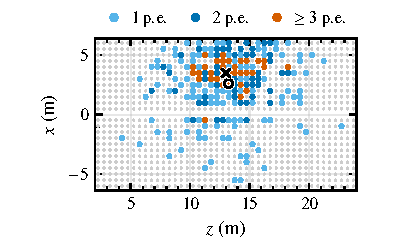
\includegraphics{figures/evento_exemplo.pdf}
    \caption{Parede longa em $y = {}$\qty{-6.673}{\m}, a mais próxima do vértice, no evento de teste \num{5834} (\qty{387}{\pe} em \num{247} dos \num{6912} canais); ela recebe a maior parte da luz, e todos os seus canais com luz estão no trecho exibido. Pontos cinza: canais sem luz; cor: fotoelétrons por canal; cruz: projeção do vértice; círculo: projeção do centroide da luz, onde fica o nó global do grafo (Seção~\ref{sec:dados_grafos}).}
    \label{fig:evento_exemplo}
  \end{subfigure}\hfill
  \begin{subfigure}[t]{0.485\textwidth}
    \centering
    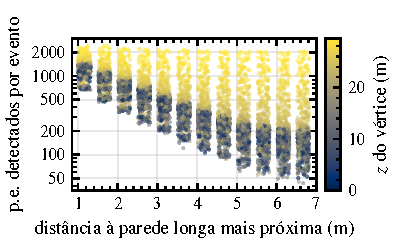
\includegraphics{figures/luz_distancia.pdf}
    \caption{Luz detectada por evento, em escala logarítmica, nos \num{9364} eventos simulados, em função da distância do vértice à parede longa mais próxima; a cor indica a coordenada $z$ do vértice. A luz cai com a distância e é maior perto da tampa. Os vértices ocupam \num{12} distâncias, a cada \qty{0.5}{\m}; os pontos foram deslocados ao acaso na horizontal para reduzir a sobreposição.}
    \label{fig:luz_distancia}
  \end{subfigure}
  \caption{Regime de contagem de fótons: (a) um evento de teste; (b) a luz de todos os eventos simulados.}
  \label{fig:regime_fotons}
\end{figure}

\subsection{Objetivo e formulação da tarefa}
\label{sec:tarefa}

Na etapa anterior \cite{vicentin2024study}, uma rede densa de \num{8195} parâmetros sobre \num{60} descritores selecionados em fases obteve erro absoluto médio (MAE) de teste de \num{12.03} a \qty{18.18}{\cm} por eixo; como os descritores resumem a leitura do detector inteiro, o modelo só recebe o que eles retêm do padrão da luz nos canais. Esta etapa representa cada evento como um grafo dos canais com luz, estima o vértice por passagem de mensagens e compara, nos mesmos eventos de teste, \num{11} codificadores com totais de parâmetros quase iguais (capacidade equiparada), \textit{boosters} ajustados (conjuntos de árvores de decisão: XGBoost e LightGBM) e o baricentro da luz, com os valores citados da rede anterior e o APEX em luz detectada igual. Procura-se ainda onde o erro se concentra e o que o limita.

A tarefa é estimar $\mathbf{v}$ com as posições $\mathbf{p}_i$ e a luz $n_i$ dos canais ativos ($n_i$ não nulo), que formam o conjunto $A$, de $|A|$ elementos.

Para o vértice previsto $\hat{\mathbf{v}}$ e $J$ eventos (\num{937} no teste), calculam-se
\begin{equation}
  \begin{aligned}
    \mathrm{MAE}_a &= \bigl\langle \lvert \hat{v}_a - v_a \rvert \bigr\rangle, &\qquad
    \mathrm{RMSE}_a &= \sqrt{\bigl\langle (\hat{v}_a - v_a)^2 \bigr\rangle}, \\
    \mathrm{RMSE}_{\mathrm{comb}} &= \sqrt{\tfrac{1}{3} \textstyle\sum_{a} \mathrm{RMSE}_a^2}, &\qquad
    \bar{d} &= \bigl\langle \lVert \hat{\mathbf{v}} - \mathbf{v} \rVert \bigr\rangle,
  \end{aligned}
  \label{eq:metricas}
\end{equation}
em que $\langle\cdot\rangle$ é a média sobre os $J$ eventos, $v_a$ e $\hat{v}_a$ são as componentes de $\mathbf{v}$ e $\hat{\mathbf{v}}$ no eixo $a \in \{x, y, z\}$, $\mathrm{MAE}_a$ e $\mathrm{RMSE}_a$ são o MAE e a raiz do erro quadrático médio (RMSE) nesse eixo, $\mathrm{RMSE}_{\mathrm{comb}}$ é o RMSE combinado, que não depende da atribuição dos eixos, e $\bar{d}$ é o erro tridimensional (3-D) médio. O MAE médio é a média dos três $\mathrm{MAE}_a$; $\bar{d}$ é também a perda do treinamento e o critério de ordenação dos codificadores.


\section{Revisão de Literatura}

\label{sec:revisao}

\subsection{Reconstrução de posição a partir da luz}
\label{sec:rev_luz}

Em detectores de líquidos nobres, a posição de um depósito é obtida do padrão de luz nos fotossensores por centroides ponderados pela luz (enviesados para o centro do arranjo), ajustes de máxima verossimilhança a funções de resposta luminosa ou redes neurais; no LUX, esse ajuste atinge \qty{0.82}{\cm} de resolução na posição horizontal com \num{200} fótons detectados de eletroluminescência (S2) no gás junto ao arranjo superior \cite{akerib2018position}. No XENONnT, redes densas, com restrição de grafo e convolucionais a estimam pelo mesmo sinal; em simulação, as duas primeiras chegam a cerca de \qty{1.5}{\cm} para S2 de aproximadamente \qty{100}{\pe} \cite{aprile2025xenonnt}. No DEAP-3600, de fase única, cada coordenada vem de uma rede densa sobre as cargas de \num{255} fotomultiplicadoras \cite{adhikari2025position}.

Em LArTPCs, a luz costuma dar o gatilho e o $t_0$ \cite{abratenko2024scintillation, paulucci2022dune}. Em simulação do FD2, o baricentro da luz tem resolução aproximadamente inversamente proporcional à raiz do número de fotoelétrons e melhor que \qty{1}{\m} em baixa energia \cite{paulucci2022dune}. No SBND, para neutrinos simulados de centenas de MeV, a posição no plano dos fotodetectores vem só da luz, com cerca de \qty{25}{\cm} de resolução no interior e vieses de até \qty{50}{\cm} na borda \cite{abratenko2024scintillation}. O APEX estima $z$ pelo baricentro das coordenadas $z_i$ dos canais ponderado pelos fotoelétrons, $\bar{z} = \sum_i n_i z_i / \sum_i n_i$; estima a coordenada horizontal pela assimetria entre a luz das duas paredes longas e a vertical por um baricentro corrigido por funções da horizontal. Sua resolução, em função da energia, é cerca de metade da obtida numa simulação semelhante do FD2 \cite{marinho2025apex}.

No JUNO, de cintilador líquido, redes convolucionais sobre os sinais de cada fotomultiplicadora reconstroem, em simulação, o vértice com cerca de \qty{10}{\cm} por eixo a \qty{1}{\MeV}, quatro vezes melhor que árvores de decisão com \textit{boosting} (Seção~\ref{sec:rev_arvores}) e redes densas sobre atributos agregados; uma rede em grafos foi aplicada só à energia \cite{qian2021vertex}.

\subsection{Redes neurais em grafos}
\label{sec:rev_gnn}

{\displaywidowpenalty=10000 \abovedisplayshortskip=\abovedisplayskip \belowdisplayshortskip=\belowdisplayskip Uma rede neural em grafos (GNN) opera num grafo $G = (\mathcal{V}, \mathcal{E})$ de nós $\mathcal{V}$ e arestas dirigidas~$\mathcal{E}$. Na camada $\ell$, a passagem de mensagens \cite{gilmer2017neural} atualiza o estado~$\mathbf{h}_i^{(\ell)}$ de cada nó~$i$,
\begin{equation}
  \mathbf{h}_i^{(\ell)} = U^{(\ell)}\Big(\mathbf{h}_i^{(\ell-1)},\ \bigoplus_{j \in \mathcal{N}(i)} M^{(\ell)}\big(\mathbf{h}_i^{(\ell-1)}, \mathbf{h}_j^{(\ell-1)}, \mathbf{e}_{ji}\big)\Big),
  \label{eq:mensagens}
\end{equation}
em que $\mathcal{N}(i)$ reúne os vizinhos de entrada de $i$, nós $j$ com aresta $(j, i)$ de atributos $\mathbf{e}_{ji}$; $M^{(\ell)}$ e $U^{(\ell)}$ são as funções de mensagem e de atualização; e $\oplus$ é uma agregação invariante à ordem. Após $L$ camadas, cada estado resume a vizinhança de até $L$ arestas, e uma leitura (\textit{readout}) invariante à ordem reduz os estados a um vetor do evento, usado na regressão. O~esquema convém a um detector, cujos canais ativos variam em número e não têm ordem.\par}

Os operadores comparados diferem na mensagem e na agregação: EdgeConv toma o máximo de uma rede aplicada ao estado e à diferença para cada vizinho \cite{wang2019dynamic}; GraphSAGE, a média \cite{hamilton2017inductive}; GINE, a soma com os atributos de aresta \cite{hu2020strategies}; GATv2, uma soma ponderada por atenção dinâmica \cite{brody2022how}; ResGatedGCN, uma soma com portas \cite{bresson2017residual}; GeneralConv, uma soma ponderada por atenção sobre mensagens com atributos de aresta \cite{you2020design}; PNA combina quatro agregadores reescalados pelo grau do nó \cite{corso2020principal}; e GPS acrescenta à passagem local uma atenção global \cite{rampasek2022recipe}. O melhor desenho muda de tarefa para tarefa \cite{you2020design}, e comparações entre arquiteturas fixam o orçamento de parâmetros, para que o tamanho do modelo não decida o resultado \cite{dwivedi2023benchmarking}.

No IceCube, a rede dynedge, baseada em EdgeConv sobre os pulsos dos módulos ópticos, reconstrói a energia, a direção e o vértice de eventos simulados entre \num{1} e \qty{30}{\GeV} com resoluções em média \num{13} a \qty{20}{\percent} melhores que as dos métodos de máxima verossimilhança \cite{abbasi2022graph}. Este trabalho aplica a mesma ideia à luz de cintilação de depósitos de \qty{10}{\MeV} no FD3.

\subsection{Árvores com \texorpdfstring{\textit{gradient boosting}}{gradient boosting}}
\label{sec:rev_arvores}

O \textit{gradient boosting} soma árvores de decisão, cada uma ajustada aos resíduos das anteriores; XGBoost e LightGBM, aqui chamados \textit{boosters}, são implementações regularizadas e rápidas \cite{chen2016xgboost, ke2017lightgbm}. Em dados tabulares de tamanho médio, conjuntos de árvores ainda superam redes profundas \cite{grinsztajn2022why}. O Optuna \cite{akiba2019optuna} escolhe hiperparâmetros por busca bayesiana com o estimador de Parzen estruturado em árvore (TPE) de \citeonline{bergstra2011algorithms}. A etapa anterior filtrou descritores por variância, correlação de distância, importância em árvores, ablação e valores de Shapley até restarem as \num{60} entradas da rede densa \cite{vicentin2024study}.


% ========== RESULTADOS OBTIDOS ==========
\section{Resultados}

\label{sec:resultados}

Como o modelo de relatório do PIBIC não inclui seção de métodos, as Seções~\ref{sec:dados_grafos} a~\ref{sec:protocolo_comparacao} descrevem os métodos desenvolvidos nesta etapa; seguem os resultados (Seções~\ref{sec:codificadores} a~\ref{sec:limites}), as dificuldades (Seção~\ref{sec:dificuldades}) e as alterações (Seção~\ref{sec:alteracoes}). Os codificadores foram treinados e avaliados na execução de 8 de agosto de 2026, e os \textit{boosters}, na de 4 de agosto. Para este relatório, sem novo treinamento, foram reavaliados os \textit{boosters} e calculados os intervalos de confiança e o baricentro $\bar{z}$.

\subsection{Dados e representação em grafos}
\label{sec:dados_grafos}

Os vértices dos nomes de arquivo não estavam no referencial dos sensores, e os \num{1152} canais das tampas tinham $y$ e $z$ com o sinal trocado; as duas correções foram aplicadas na construção da base de dados e conferidas nos \num{9364} eventos. Três canais quentes, com contagem em todos os eventos e \qty{47.1}{\percent} das contagens brutas, foram substituídos pela média dos vizinhos sãos: a base guarda a luz já corrigida. Uma posição foi simulada duas vezes, e três arquivos eram cópias de outros. Depois das correções, o centroide da luz detectada acompanha o vértice, com coeficiente de correlação de Pearson $r$ de \num{0.908} em $x$, \num{0.871} em $y$ e \num{0.999} em $z$ nos \num{9364} eventos.

Os eventos foram divididos em \num{7490} de treino, \num{937} de validação e \num{937} de teste, estratificados em \num{9} faixas por eixo (\num{729} grupos), divisão comum a todos os modelos. Pela simetria dos canais sob trocas de sinal dos eixos, cada evento de treino foi espelhado nos outros octantes: \num{56884} linhas de treino, \num{7.59} por evento; os de validação e de teste ficam no octante simulado. Os vértices de teste distam, em média, \qty{49.31}{\cm} do vértice de treino mais próximo e, salvo a posição simulada duas vezes, são posições da grade ausentes do treino: os erros medem interpolação numa grade de \qty{0.5}{\m}, com um sorteio de fótons por evento.

Os nós do grafo $G = (\mathcal{V}, \mathcal{E})$ são os $|A|$ canais ativos do evento, \num{245} em média nos eventos de teste, e um nó global \cite{gilmer2017neural} no centroide da luz. Cada canal recebe arestas dos $k = {}$\num{4} canais ativos mais próximos, num grafo de $k$ vizinhos mais próximos (\mbox{$k$-NN}), e troca uma aresta em cada sentido com o nó global: seis arestas dirigidas por canal (\num{248} nós e \num{1482} arestas no evento da Figura~\ref{fig:evento_exemplo}). Cada nó $i$ tem \num{17} atributos $\mathbf{f}_i$: posição, luz, fração da luz, distância e direção ao centroide, direção ao canal mais claro, luz dos vizinhos, autovalores da matriz de covariância das posições ponderada pela luz (comuns a todos os nós do evento) e posto da luz. Cada aresta tem \num{23} atributos $\mathbf{e}_{ji}$: distância, direção, inverso do quadrado da distância, diferença e semelhança de luz, e \num{16} funções de base radial da distância até \qty{7}{\m}. Os \num{33} escalares do evento, $\mathbf{u}$, são centroides com peso linear e quadrático, luz total, número de canais ativos, maior luz de canal, dispersões, assimetrias e quantis da posição. As normalizações usam só o treino (\num{8192} grafos amostrados), e cada coordenada do vértice é padronizada.

\subsection{Codificadores e protocolo de treinamento}
\label{sec:modelos}

Os modelos (Figura~\ref{fig:arquitetura}) projetam os \num{17} atributos $\mathbf{f}_i$ de cada nó num estado inicial $\mathbf{h}_i^{(0)}$ de largura $D$ e aplicam $L = {}$\num{4} camadas residuais,
\begin{equation}
  \mathbf{h}_i^{(\ell)} = \mathbf{h}_i^{(\ell-1)} + \mathrm{GELU}\Big(\mathrm{Conv}^{(\ell)}\big(\mathrm{LN}^{(\ell)}(\mathbf{h}_i^{(\ell-1)}),\ \{(\mathrm{LN}^{(\ell)}(\mathbf{h}_j^{(\ell-1)}),\, \mathbf{e}_{ji})\}_{j \in \mathcal{N}(i)}\big)\Big), \quad \ell = 1, \dots, L,
  \label{eq:camada}
\end{equation}
com normalização de camada $\mathrm{LN}^{(\ell)}$ de \citeonline{ba2016layer}, ativação GELU (unidade linear de erro gaussiano) de \citeonline{hendrycks2016gaussian} e operador $\mathrm{Conv}^{(\ell)}$, que lê $\mathbf{e}_{ji}$, exceto em EdgeConv, GraphSAGE e ResGatedGCN. Nos GPS, uma porta aprendida mistura um GATv2 local, sem GELU, e uma atenção global; um bloco denso residual completa a camada. A leitura concatena média, máximo e soma comprimida por logaritmo dos estados. Os \num{33} escalares $\mathbf{u}$ entram na cabeça de regressão diretamente e também codificados em \num{128} dimensões. A cabeça prevê $x$, depois $y$ dado o $x$ previsto e $z$ dados os $x$ e $y$ previstos, mesmo no treino, por modulação linear por atributo (FiLM) de \citeonline{perez2018film} ou, nos modelos de sufixo cascata, por concatenação; o sufixo designa só a cabeça. Uma limitação suave mantém a predição na caixa \textpm(\num{6.03};~\num{6.67};~\num{29.93})\,\unit{\m}, com inclinação pequena fora dela.

\begin{figure}[H]
  \centering
  \begin{tikzpicture}[
  x=1cm, y=1cm,
  line width=0.45pt,
  flow/.style={-latex, line width=0.45pt},
  knn/.style={line width=0.35pt},
  spoke/.style={line width=0.35pt, draw=black!45},
  channel/.style={circle, fill=black, inner sep=0pt, minimum size=1.2mm},
  globalnode/.style={circle, fill=black!45, inner sep=0pt, minimum size=2.2mm},
  branch/.style={circle, fill=black, inner sep=0pt, minimum size=0.8mm},
  txt/.style={inner sep=0pt, anchor=base},
  dag/.style={inner sep=1.6pt, execute at begin node={\vphantom{$\hat{x}\hat{y}\hat{z}$}}}
]
\def\arqrowa{3.28}
\def\arqrowb{0.92}
\def\arqgap{2.14}
\def\arqtop{4.22}

\coordinate (g)  at (1.45, 3.20);
\coordinate (c0) at (2.41, 3.42);
\coordinate (c1) at (1.85, 3.94);
\coordinate (c2) at (1.32, 3.92);
\coordinate (c3) at (0.54, 3.65);
\coordinate (c4) at (0.55, 2.91);
\coordinate (c5) at (1.01, 2.50);
\coordinate (c6) at (1.68, 2.45);
\coordinate (c7) at (2.25, 2.80);

\foreach \i in {0,...,7} {\draw[spoke] (g) -- (c\i);}
\foreach \i/\j in {0/1,1/2,2/3,3/4,4/5,5/6,6/7,7/0,0/2,1/3,2/4,3/5,4/6,5/7,6/0,7/1} {\draw[knn] (c\i) -- (c\j);}
\foreach \i in {0,...,7} {\node[channel] at (c\i) {};}
\node[globalnode] at (g) {};
\node[txt] at (1.45, \arqtop) {grafo do evento};

\draw[flow] (2.57, \arqrowa) -- (2.95, \arqrowa);
\draw (2.95, \arqrowa-0.50) rectangle (5.10, \arqrowa+0.50);
\node[txt] at (4.025, \arqrowa+0.10) {projeção};
\node[txt] at (4.025, \arqrowa-0.40) {\num{17} $\to$ $D$};

\draw (5.50, \arqrowa-0.50) rectangle (11.95, \arqrowa+0.78);
\node[txt] at (8.725, \arqtop) {\num{4} camadas residuais};
\draw[flow] (5.10, \arqrowa) -- (6.15, \arqrowa);
\node[branch] at (5.72, \arqrowa) {};
\draw[flow] (5.72, \arqrowa) -- (5.72, \arqrowa+0.50) -- (11.55, \arqrowa+0.50) -- (11.55, \arqrowa+0.16);
\draw (6.15, \arqrowa-0.27) rectangle (6.95, \arqrowa+0.27);
\node[txt] at (6.55, \arqrowa-0.12) {LN};
\draw[flow] (6.95, \arqrowa) -- (7.35, \arqrowa);
\draw (7.35, \arqrowa-0.27) rectangle (9.25, \arqrowa+0.27);
\node[txt] at (8.30, \arqrowa-0.12) {operador};
\draw[flow] (9.25, \arqrowa) -- (9.65, \arqrowa);
\draw (9.65, \arqrowa-0.27) rectangle (11.00, \arqrowa+0.27);
\node[txt] at (10.325, \arqrowa-0.12) {GELU};
\draw[flow] (11.00, \arqrowa) -- (11.39, \arqrowa);
\draw (11.55, \arqrowa) circle (0.16);
\draw (11.44, \arqrowa) -- (11.66, \arqrowa);
\draw (11.55, \arqrowa-0.11) -- (11.55, \arqrowa+0.11);
\draw[flow] (11.71, \arqrowa) -- (12.35, \arqrowa);

\draw (12.35, \arqrowa-0.78) rectangle (15.65, \arqrowa+0.78);
\node[txt] at (14.00, \arqrowa+0.38) {leitura};
\node[txt] at (14.00, \arqrowa-0.12) {média, máximo};
\node[txt] at (14.00, \arqrowa-0.62) {e log da soma};

\draw[flow] (12.80, \arqrowa-0.78) -- (12.80, \arqgap) -- (7.225, \arqgap) -- (7.225, \arqrowb+0.66) -- (7.60, \arqrowb+0.66);

\node[txt] at (1.45, \arqrowb+0.88) {escalares};
\node[txt] at (1.45, \arqrowb+0.38) {do evento};
\node[txt] at (1.45, \arqrowb-0.12) {$\mathbf{u}$ (\num{33})};
\draw[flow] (2.05, \arqrowb) -- (2.95, \arqrowb);
\node[branch] at (2.50, \arqrowb) {};
\draw[flow] (2.50, \arqrowb) -- (2.50, \arqrowb-0.66) -- (7.60, \arqrowb-0.66);
\draw (2.95, \arqrowb-0.50) rectangle (5.10, \arqrowb+0.50);
\node[txt] at (4.025, \arqrowb+0.10) {projeção};
\node[txt] at (4.025, \arqrowb-0.40) {\num{33} $\to$ \num{128}};
\draw[flow] (5.10, \arqrowb) -- (5.50, \arqrowb);
\draw (5.50, \arqrowb-0.27) rectangle (6.85, \arqrowb+0.27);
\node[txt] at (6.175, \arqrowb-0.12) {GELU};
\draw[flow] (6.85, \arqrowb) -- (7.60, \arqrowb);

\draw (7.60, \arqrowb-0.90) rectangle (12.60, \arqrowb+0.90);
\node[txt] at (10.10, \arqrowb+0.50) {cabeça};
\node[dag] (xh) at (9.20, \arqrowb-0.14) {$\hat{x}$};
\node[dag] (yh) at (10.10, \arqrowb-0.14) {$\hat{y}$};
\node[dag] (zh) at (11.00, \arqrowb-0.14) {$\hat{z}$};
\draw[flow] (xh) -- (yh);
\draw[flow] (yh) -- (zh);
\draw[flow] (xh.north) to[bend left=20] (zh.north);
\node[txt] at (10.10, \arqrowb-0.72) {FiLM ou concatenação};
\draw[flow] (12.60, \arqrowb) -- (13.00, \arqrowb);

\draw (13.00, \arqrowb-0.90) rectangle (15.00, \arqrowb+0.90);
\node[txt] at (14.00, \arqrowb+0.50) {limitação};
\node[txt] at (14.00, \arqrowb) {suave};
\draw (13.40, \arqrowb-0.70) -- (13.75, \arqrowb-0.66) -- (14.25, \arqrowb-0.24) -- (14.60, \arqrowb-0.20);
\draw[flow] (15.00, \arqrowb) -- (15.40, \arqrowb);
\node[txt, anchor=base west] at (15.45, \arqrowb-0.12) {$\hat{\mathbf{v}}$ (m)};
\end{tikzpicture}\relax

  \caption{Estrutura comum aos \num{11} codificadores. O grafo do evento tem um nó por canal ativo e um nó global no centroide da luz; quatro camadas residuais atualizam os estados dos nós, que a leitura resume em média, máximo e soma comprimida por logaritmo; a cabeça recebe também os \num{33} escalares do evento e prevê $x$, depois $y$ dado o $x$ previsto ($\hat{x}$) e $z$ dados $\hat{x}$ e o $y$ previsto ($\hat{y}$); a limitação suave mantém o vértice previsto $\hat{\mathbf{v}}$, em metros, na caixa definida pelos canais. Entre os codificadores mudam só o operador (nos GPS, a camada inteira), a largura $D$ e, nos modelos de sufixo cascata, a cabeça.}
  \label{fig:arquitetura}
\end{figure}

A largura $D$ de cada codificador foi escolhida \cite{dwivedi2023benchmarking} para aproximar o total de parâmetros do GPS, \num{1843395}. Dos \num{14} codificadores dimensionados, \num{11} foram treinados (Seção~\ref{sec:dificuldades}), com \num{1819019} a \num{1873531} parâmetros (desvio máximo de \qty{1.6}{\percent}) e $D$ de \num{132} a \num{685}, exceto no GPS (Tabela~\ref{tab:codificadores}). A capacidade equiparada é a do modelo inteiro: a parcela do codificador vai de \qty{58.3}{\percent} (EdgeConv) a \qty{85.4}{\percent} (\mbox{GPS-cascata}).

A perda $\mathcal{L}$ é a distância euclidiana média, em metros, entre o vértice previsto $\hat{\mathbf{v}}_b$ e o verdadeiro $\mathbf{v}_b$ das $B$ linhas $b$ do lote,
\begin{equation}
  \mathcal{L} = \frac{1}{B} \sum_{b=1}^{B} \big\lVert \hat{\mathbf{v}}_b - \mathbf{v}_b \big\rVert,
  \label{eq:perda}
\end{equation}
a mesma grandeza do erro 3-D médio. O otimizador AdamW \cite{loshchilov2019decoupled} usou coeficientes das médias móveis de \num{0.9} e \num{0.999}, decaimento de pesos de \num{e-4} no codificador e \num{e-5} na cabeça, e taxas de aprendizado de \num{5e-4} e \num{5e-3}, respectivamente, para lotes de \num{128} (\num{1.5e-4} e \num{1.5e-3} nos GPS), multiplicadas por $B$/\num{128} \cite{goyal2017accurate}. O lote $B$ foi a maior potência de dois, até \num{512}, que coube em \qty{20}{\gibi\byte} numa sonda de memória: \num{128} em quatro modelos, \num{256} em dois e \num{512} em cinco. Houve aquecimento linear de \num{100} passos de otimização a partir de \num{0.1} vez a taxa, decaimento cossenoidal até \num{e-6} em \num{50} épocas \cite{loshchilov2017sgdr} e limitação da norma do gradiente em \num{1.0}. O teste usou o ponto de verificação de menor erro de validação; não houve precisão mista, aumento de dados além do espelhamento nem média móvel dos pesos. Cada codificador foi treinado uma vez, com semente \num{42}, sem busca de hiperparâmetros. Os treinos somaram \qty{11.42}{\hour} numa unidade de processamento gráfico (GPU) de \qty{23.98}{\gibi\byte}, com \num{5600} a \num{22250} passos: a capacidade foi equiparada, mas o orçamento de otimização variou.

\subsection{Referências e incerteza das comparações}
\label{sec:protocolo_comparacao}

Nas linhas de treino dos codificadores, XGBoost e LightGBM \cite{chen2016xgboost,ke2017lightgbm} ajustam por mínimos quadrados um regressor por coordenada a \num{58} atributos agregados, como centroides com peso linear e quadrático, quantis, dispersões, assimetrias e canais mais claros. Cada regressor tem até \num{3000} árvores, com parada após \num{100} rodadas sem melhora na validação; os hiperparâmetros são os de menor erro 3-D médio de validação em \num{40} tentativas de TPE, \num{12} delas aleatórias \cite{akiba2019optuna}. Nos registros, a validação e o teste usaram luz com aumento de dados (perda e ativação espúria de canais, ruído, variação de ganho, afinamento de fótons), com \qty{4.1}{\percent} menos luz no teste. Este relatório reavalia os \textit{boosters} na luz limpa dos codificadores; com aumento, reproduz exatamente os valores registrados. A~busca e o treino, porém, usaram luz com aumento.

A rede da etapa anterior \cite{vicentin2024study} é citada, não reavaliada: usou outra partição (\qty{80}{\percent} e \qty{20}{\percent}), a geometria anterior à correção das tampas e, a julgar pelos gráficos, o referencial dos nomes de arquivo. O APEX \cite{marinho2025apex} usa outra simulação (\qty{10}{ppm} de xenônio, refletividade de \qty{79}{\percent} na gaiola de campo, luz reemitida pelos fotodetectores) e estimadores analíticos. Suas larguras de resolução nos próprios eixos, $\sigma_x$, $\sigma_y$ e $\sigma_z$, lidas da Figura~2 do artigo a \qty{0.26}{\cm} por \textit{pixel}, não têm definição publicada; a largura combinada $\sigma_{\mathrm{comb}}$ é a média quadrática delas. A comparação principal é em luz detectada igual, que não garante igual informação de posição: os \qty{530.1}{\pe}\ médios do teste equivalem a \qty{2.9}{\MeV} no APEX com o rendimento médio, \qty{180}{\pe\per\MeV}, e a \qty{4.9}{\MeV} com o mínimo, \qty{109}{\pe\per\MeV}, energia em que até a região mais escura do APEX dá essa luz, o que favorece o APEX; também se compara em energia igual, \qty{10}{\MeV}. Só $\sigma_{\mathrm{comb}}$ e $\sigma_z$ são comparados: a correspondência das larguras transversais com $x$ e $y$ não está estabelecida.

O baricentro $\bar{z}$, com calibração quadrática ajustada em \num{4000} eventos de treino sorteados, usa os mesmos \num{937} eventos de teste e o mesmo sorteio de fótons. Os intervalos de \qty{95}{\percent} vêm de reamostragem \textit{bootstrap} dos eventos de teste \cite{efron1979bootstrap}, pareada nos codificadores e \textit{boosters}, com \num{10000} reamostras comuns, e não pareada no baricentro, com \num{2000}; cobrem a amostragem do teste, não a variação entre treinos. Como os mesmos eventos de teste serviram à primeira comparação e ao diagnóstico que orientou a final (Seção~\ref{sec:dificuldades}), os erros de teste dos codificadores podem ser algo otimistas, o que os intervalos também não cobrem. Diferenças, razões e porcentagens são calculadas sem arredondamento.

\subsection{Comparação entre os codificadores}
\label{sec:codificadores}

No teste, os \num{11} codificadores ficam entre \num{25.95} e \qty{28.83}{\cm} de erro 3-D médio, faixa de \qty{2.89}{\cm}, com MAE médio de \num{12.63} a \qty{14.14}{\cm} e RMSE combinado de \num{18.55} a \qty{20.64}{\cm} (Tabela~\ref{tab:codificadores}). Os quatro primeiros, GATv2-cascata (\qty{25.95}{\cm}), GPS-cascata (\qty{26.06}{\cm}), GATv2 (\qty{26.08}{\cm}) e GPS (\qty{26.27}{\cm}), diferem em até \qty{0.32}{\cm}.

\begin{table}[H]
  \centering
  \caption{Os \num{11} codificadores da comparação final, com capacidade equiparada a \num{1843395} parâmetros, em ordem crescente de erro 3-D médio nos \num{937} eventos de teste; MAE médio, RMSE combinado e erro 3-D médio em cm. $D$: largura dos estados dos nós; $B$: lote escolhido pela sonda de memória (\num{128}, \num{256} ou \num{512} linhas de treino espelhadas, que correspondem, respectivamente, a \num{22250}, \num{11150} e \num{5600} passos de otimização em \num{50} épocas), com as taxas de aprendizado multiplicadas por $B$/\num{128}. $^{\dagger}$: não lê os atributos das arestas. Os quatro primeiros não se distinguem pela reamostragem pareada (Figura~\ref{fig:diferenca_pareada}).}
  \label{tab:codificadores}
  \begin{tabular}{@{}l S[table-format=3.0] S[table-format=1.3] S[table-format=3.0] S[table-format=2.2] S[table-format=2.2] S[table-format=2.2]@{}}
\toprule
 & {} & {Parâmetros} & {} & {MAE} & {RMSE} & {Erro 3-D} \\
Codificador & {$D$} & {(\num{e6})} & {$B$} & {médio (cm)} & {comb.\ (cm)} & {médio (cm)} \\
\midrule
GATv2-cascata & 212 & 1.869 & 128 & 12.63 & 18.64 & 25.95 \\
GPS-cascata & 132 & 1.874 & 128 & 12.79 & 18.69 & 26.06 \\
GATv2 & 204 & 1.819 & 128 & 12.74 & 18.80 & 26.08 \\
GPS & 128 & 1.843 & 256 & 12.95 & 18.55 & 26.27 \\
GeneralConv & 280 & 1.833 & 256 & 12.86 & 18.94 & 26.43 \\
ResGatedGCN$^{\dagger}$ & 292 & 1.841 & 512 & 13.07 & 19.02 & 26.71 \\
GraphSAGE$^{\dagger}$ & 400 & 1.840 & 512 & 13.23 & 19.01 & 26.92 \\
EdgeConv$^{\dagger}$ & 685 & 1.843 & 128 & 13.46 & 20.23 & 27.67 \\
PNA & 147 & 1.841 & 512 & 13.52 & 19.57 & 27.68 \\
GINE & 395 & 1.844 & 512 & 13.81 & 20.21 & 28.23 \\
GINE-cascata & 404 & 1.843 & 512 & 14.14 & 20.64 & 28.83 \\
\bottomrule
\end{tabular}

\end{table}

As diferenças pareadas do erro 3-D médio em relação ao GATv2-cascata são de \qty[retain-explicit-plus]{+0.12}{\cm} (\num{-0.30} a \qty{0.54}{\cm}) para o GPS-cascata, \qty[retain-explicit-plus]{+0.13}{\cm} (\num{-0.28} a \qty{0.55}{\cm}) para o GATv2 e \qty[retain-explicit-plus]{+0.32}{\cm} (\num{-0.12} a \qty{0.77}{\cm}) para o GPS, intervalos que contêm o zero; do GeneralConv em diante (\qty[retain-explicit-plus]{+0.48}{\cm}; \num{0.02} a \qty{0.95}{\cm}), os intervalos ficam acima de zero, sem correção para comparações múltiplas (Figura~\ref{fig:diferenca_pareada}). O GATv2-cascata tem o menor erro 3-D médio em \qty{56.9}{\percent} das reamostras; o GPS, com o menor RMSE combinado (\qty{18.55}{\cm}), lidera essa métrica em \qty{61.8}{\percent} delas; o menor erro de validação é do GATv2 (\qty{25.72}{\cm}). Não há, portanto, um melhor codificador estabelecido. A seguir, o GATv2-cascata representa o grupo dos quatro melhores; foi escolhido pela métrica de teste, o que favorece seu erro de teste, e treinado uma vez, como os demais.

A parada antecipada (\num{15} épocas sem melhora na validação) não foi acionada; o menor erro de validação ocorreu entre as épocas \num{41} e \num{50}, na última época no GraphSAGE e no GeneralConv. No GATv2-cascata (Figura~\ref{fig:curvas_validacao}), o erro de treino nas linhas espelhadas termina em \qty{21.91}{\cm}, e os erros de validação e de teste concordam (\num{25.96} e \qty{25.95}{\cm}).

\begin{figure}[H]
  \centering
  \begin{subfigure}[t]{0.485\textwidth}
    \centering
    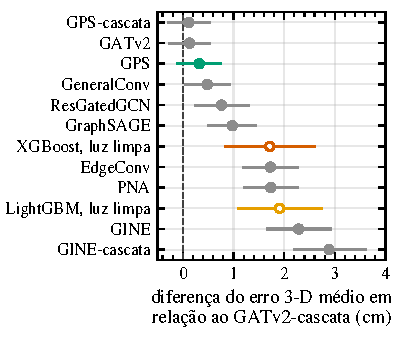
\includegraphics{figures/diferenca_pareada.pdf}
    \caption{Diferença do erro 3-D médio de teste em relação ao do GATv2-cascata, com intervalo de \qty{95}{\percent} por reamostragem \textit{boot\-strap} pareada (\num{10000} reamostras dos \num{937} eventos de teste); o GPS, de menor RMSE combinado, em verde; \mbox{XGBoost} e \mbox{LightGBM} na luz limpa, com marcador vazado. Diferenças positivas indicam erro maior que o do GATv2-cascata; os intervalos do GPS-cascata, do GATv2 e do GPS contêm o zero.}
    \label{fig:diferenca_pareada}
  \end{subfigure}\hfill
  \begin{subfigure}[t]{0.485\textwidth}
    \centering
    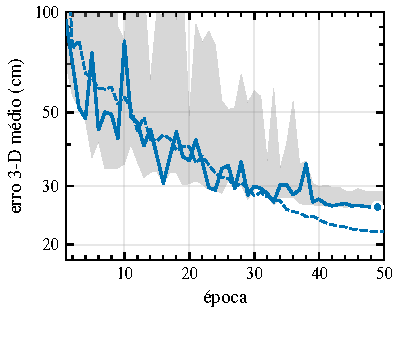
\includegraphics{figures/curvas_validacao.pdf}
    \caption{Erro 3-D médio por época, em escala logarítmica: faixa sombreada entre o menor e o maior erro de validação dos \num{11} codificadores e, para o GATv2-cascata, as curvas de validação (contínua) e de treino nas linhas espelhadas (tracejada), com marcador na época de menor erro de validação. Ficam acima da escala o valor de treino da primeira época e o limite superior da faixa em várias épocas da primeira metade do treino.}
    \label{fig:curvas_validacao}
  \end{subfigure}
  \caption{Comparação entre os \num{11} codificadores com capacidade equiparada: (a) diferenças nos \num{937} eventos de teste; (b) curvas de treinamento.}
  \label{fig:par_codificadores}
\end{figure}

Os três codificadores que não leem os atributos das arestas ficam no meio da Tabela~\ref{tab:codificadores}: ResGatedGCN em sexto, GraphSAGE em sétimo e EdgeConv em oitavo. Os cinco treinados com lote \num{512} (\num{5600} passos) ocupam as posições 6, 7, 9, 10 e 11, e os três primeiros usaram lote \num{128} (\num{22250} passos): a comparação iguala o número de parâmetros, mas não separa o efeito do operador do efeito do orçamento de otimização.

\subsection{Comparação com as referências}
\label{sec:comparacao_referencias}

Na luz limpa, o GATv2-cascata tem erro 3-D médio \qty{1.71}{\cm} menor que o do XGBoost (\num{0.83} a \qty{2.62}{\cm}) e RMSE combinado \qty{2.30}{\cm} menor (\num{1.66} a \qty{2.95}{\cm}); contra o LightGBM, \num{1.91} e \qty{1.98}{\cm} (Figura~\ref{fig:diferenca_pareada} e Tabela~\ref{tab:referencias}). Pelas estimativas pontuais, sete dos \num{11} codificadores têm erro 3-D médio menor que o do XGBoost, mas o GATv2-cascata fica mais perto do vértice que o XGBoost em só \qty{47.6}{\percent} dos eventos: o XGBoost erra menos nos eventos mais claros, e o GATv2-cascata, nos mais escuros e na cauda, com percentil 90 do erro 3-D de \qty{51.26}{\cm} contra \qty{60.26}{\cm} (Seção~\ref{sec:onde_erro}). Nos registros das execuções, em luz com aumento, o XGBoost tem MAE médio de \qty{13.01}{\cm} e RMSE combinado de \qty{20.82}{\cm}, contra \num{13.21} e \qty{20.95}{\cm} na luz limpa.

Em relação à rede da etapa anterior \cite{vicentin2024study}, com valores obtidos em outra partição e na geometria anterior às correções, o RMSE combinado do GATv2\discretionary{-}{-}{-}cascata é \qty{10.6}{\percent} menor (\num{18.64} contra \qty{20.86}{\cm}) e o MAE médio, \qty{16.5}{\percent} menor (\num{12.63} contra \qty{15.13}{\cm}). Por eixo, no referencial dos sensores, o RMSE cai \num{4.23} e \qty{1.81}{\cm} em $x$ e $y$, e em $z$ o valor daquela rede, \qty{0.41}{\cm} maior, fica dentro do intervalo de \qty{95}{\percent} do GATv2\discretionary{-}{-}{-}cascata. Na luz limpa, os \textit{boosters} ficam a até \qty{0.24}{\cm} do RMSE combinado daquela rede, e os \num{11} codificadores, abaixo dele, entre \num{18.55} e \qty{20.64}{\cm}; para o EdgeConv, o GINE e o GINE\discretionary{-}{-}{-}cascata, como para os \textit{boosters}, o valor daquela rede fica dentro do intervalo de \qty{95}{\percent}.

\begin{table}[H]
  \centering
  \caption{Erros de teste do GATv2-cascata, do GPS e das referências, em cm, no referencial dos sensores; o baricentro tem calibração quadrática. \textsuperscript{a}RMSE por eixo citados, de outra partição (\qty{80}{\percent} e \qty{20}{\percent}) e da geometria anterior às correções \cite{vicentin2024study}, com eixos convertidos para este referencial; RMSE combinado e MAE médio calculados a partir dos valores publicados por eixo. \textsuperscript{\smash{b}}Outra simulação \cite{marinho2025apex}; larguras lidas da Figura~2 do artigo a \qty{0.26}{\cm} por \textit{pixel}, em luz detectada igual com o rendimento médio (\qty{2.9}{\MeV}) ou com o mínimo (\qty{4.9}{\MeV}) e em energia igual (\qty{10}{\MeV}); as duas larguras transversais aparecem na mesma célula, sem atribuição a $x$ e $y$; MAE não disponível.}
  \label{tab:referencias}
  \begin{tabular}{@{}l S[table-format=2.2] S[table-format=2.2] S[table-format=2.2] S[table-format=2.2] S[table-format=2.2]@{}}
\toprule
 & {RMSE $x$} & {RMSE $y$} & {RMSE $z$} & {RMSE} & {MAE} \\
Estimador & {(cm)} & {(cm)} & {(cm)} & {comb.\ (cm)} & {médio (cm)} \\
\midrule
GATv2-cascata & 20.45 & 14.35 & 20.46 & 18.64 & 12.63 \\
GPS & 20.55 & 14.29 & 20.15 & 18.55 & 12.95 \\
\midrule
XGBoost, luz limpa & 23.82 & 16.96 & 21.47 & 20.95 & 13.21 \\
LightGBM, luz limpa & 23.91 & 16.55 & 20.75 & 20.62 & 13.38 \\
Baricentro (só $z$) &  &  & 42.45 &  &  \\
\midrule
Rede densa (2024)\textsuperscript{a} & 24.68 & 16.16 & 20.87 & 20.86 & 15.13 \\
APEX, \qty{2.9}{\MeV}\textsuperscript{b} & \multicolumn{2}{c}{\num{33.1} e \num{51.3}} & 24.8 & 38.0 &  \\
APEX, \qty{4.9}{\MeV}\textsuperscript{b} & \multicolumn{2}{c}{\num{26.8} e \num{44.0}} & 19.4 & 31.8 &  \\
APEX, \qty{10}{\MeV}\textsuperscript{b} & \multicolumn{2}{c}{\num{20.8} e \num{37.3}} & 13.7 & 25.9 &  \\
\bottomrule
\end{tabular}

\end{table}

Em luz detectada igual à média do teste e com o rendimento médio, a largura combinada do APEX \cite{marinho2025apex} é de \qty{38.0}{\cm}, e o RMSE combinado do GATv2-cascata, \qty{18.64}{\cm} (\num{17.69} a \qty{19.61}{\cm}), é \qty{51.0}{\percent} menor; com o rendimento mínimo, é \qty{41.3}{\percent} menor que a largura de \qty{31.8}{\cm}, e em energia igual, \qty{28.0}{\percent} menor que a de \qty{25.9}{\cm} (Figura~\ref{fig:apex_luz}). Em $z$, contra \num{20.15} a \qty{20.46}{\cm} dos quatro melhores, o APEX tem \qty{24.8}{\cm} com o rendimento médio, acima do intervalo de \qty{95}{\percent} de cada um, e \qty{19.4}{\cm} com o mínimo, dentro dele; só em energia igual (\qty{13.7}{\cm}) é melhor. O artigo não define a largura: a \qty{4}{\MeV}, o valor do gráfico é \num{0.96} vez o desvio-padrão e \num{1.13} vez a largura gaussiana dos resíduos em $z$; uma largura gaussiana, menor que o desvio-padrão, favoreceria o APEX frente a um RMSE.

{\clubpenalty=10000 Nos mesmos eventos, o baricentro $\bar{z}$ \cite{marinho2025apex}, aqui com calibração quadrática, tem RMSE em $z$ de \qty{42.45}{\cm} (\num{39.55} a \qty{45.22}{\cm}; \qty[uncertainty-mode = separate, separate-uncertainty-units = single]{41.98 \pm 0.61}{\cm}, média e desvio-padrão em \num{30} sorteios de fótons; Figura~\ref{fig:baricentro_luz}), \num{2.07} vezes o do GATv2-cascata, e com calibração cúbica, \qty{41.86}{\cm}. Sem calibração, o baricentro tem \qty{66.59}{\cm}, deslocado em média \qty{34.08}{\cm} para a tampa mais próxima, sobretudo nos vértices a partir de $z = {}$\qty{20}{\m} (Seção~\ref{sec:onde_erro}), viés não encontrado no APEX. Dos estimadores de uma só estatística testados, o baricentro de todos os canais é o melhor (com calibração cúbica, só dos canais a mais de \qty{1}{\m} das tampas: \qty{66.95}{\cm}; canal mais claro: \qty{142.16}{\cm}).\par}

\begin{figure}[H]
  \centering
  \begin{subfigure}[t]{0.485\textwidth}
    \centering
    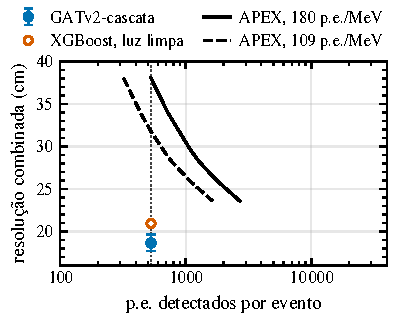
\includegraphics{figures/apex_luz.pdf}
    \caption{Largura combinada do APEX em outra simulação \cite{marinho2025apex}, com a energia convertida em fotoelétrons pelo rendimento médio (\qty{180}{\pe\per\MeV}; \qty{10}{\MeV} dão \qty{1800}{\pe}) e pelo mínimo (\qty{109}{\pe\per\MeV}), e RMSE combinado do GATv2-cascata (intervalo de \qty{95}{\percent}) e do \mbox{XGBoost} em luz limpa, na luz média do teste (\qty{530.1}{\pe}, linha pontilhada).}
    \label{fig:apex_luz}
  \end{subfigure}\hfill
  \begin{subfigure}[t]{0.485\textwidth}
    \centering
    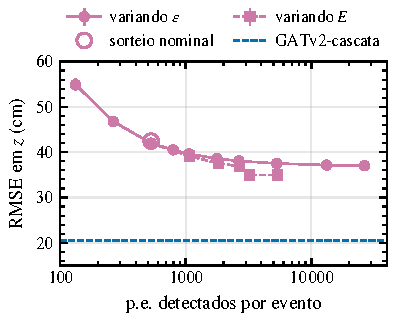
\includegraphics{figures/baricentro_luz.pdf}
    \caption{RMSE em $z$ do baricentro com calibração quadrática no teste, ao variar a eficiência $\varepsilon$ de \num{0.005} a \num{1}, com $E$ fixa em \qty{10}{\MeV}, ou a energia $E$ de \num{10} a \qty{100}{\MeV}, com $\varepsilon$ fixa em \num{0.02}: média de \num{30} sorteios de fótons e desvio-padrão (barras, menores que os marcadores, exceto em $\varepsilon = {}$\num{0.005}); círculo vazado: sorteio nominal, usado no treino e no teste dos modelos; linha horizontal: GATv2\discretionary{-}{-}{-}cascata, avaliado só nesse sorteio.}
    \label{fig:baricentro_luz}
  \end{subfigure}
  \caption{Resolução, em função da luz detectada por evento, dos estimadores analíticos e, só na luz do teste, dos modelos: (a) combinada nos três eixos; (b) em $z$.}
  \label{fig:par_luz_referencias}
\end{figure}

\subsection{Onde o erro se concentra}
\label{sec:onde_erro}

O erro 3-D por evento cai com a luz detectada: a correlação de postos de Spearman $\rho_{\mathrm{S}}$ vale \num{-0.68} no GATv2-cascata e \num{-0.72} no XGBoost na luz limpa. Por quartil de luz do teste (limites: \num{201}, \num{387} e \qty{773}{\pe}), o erro 3-D médio do GATv2-cascata é de \num{42.79}, \num{31.25}, \num{18.19} e \qty{11.67}{\cm}, e o do XGBoost, de \num{47.28}, \num{35.74}, \num{20.78} e \qty{6.98}{\cm} (Figura~\ref{fig:erro_luz}): o GATv2-cascata erra menos nos três mais escuros (diferenças pareadas com intervalos acima de zero), e o XGBoost, \qty{4.70}{\cm} menos no mais claro (\num{3.58} a \qty{5.75}{\cm}). Os centroides com peso quadrático e linear respondem, respectivamente, por \num{43.5} e \qty{33.3}{\percent} da importância por ganho do XGBoost, treinado em luz com aumento. Como ambos ganham precisão com a luz, isso condiz com a vantagem nos eventos claros, mas não a explica: o GATv2\discretionary{-}{-}{-}cascata recebe os mesmos dois centroides entre os escalares do evento (Seção~\ref{sec:dados_grafos}), e a causa de seu erro maior nesses eventos não foi investigada.

No referencial dos sensores, o eixo $y$, normal às paredes longas, tem o menor RMSE no GATv2-cascata (\qty{14.35}{\cm}, contra \num{20.45} e \qty{20.46}{\cm} em $x$ e $z$), no GPS, nos \textit{boosters} na luz limpa e na rede da etapa anterior (eixos convertidos por correspondência inferida; Tabela~\ref{tab:referencias}). O eixo $x$, normal às faces sem canais, tem o maior nos \textit{boosters} (XGBoost: \qty{23.82}{\cm}) e naquela rede (\qty{24.68}{\cm}). O coeficiente de determinação $R^2$ do GATv2-cascata em $z$, fração da variância explicada, é \num{0.9994} porque o desvio-padrão dos vértices de teste é \num{4.6} vezes maior em $z$ que em $x$, não porque $z$ seja mais bem reconstruído.

Abaixo de $z = {}$\qty{20}{\m} (\num{626} eventos), os RMSE em $z$ do baricentro calibrado, do GATv2\discretionary{-}{-}{-}cascata e do XGBoost na luz limpa são próximos (\num{23.29}, \num{22.54} e \qty{22.63}{\cm}); a partir de \qty{20}{\m} (\num{311} eventos), o do baricentro sobe para \qty{65.87}{\cm}, e os outros dois caem para \num{15.44} e \qty{18.91}{\cm} (Figura~\ref{fig:erro_z}). O fator \num{2.07} da Seção~\ref{sec:comparacao_referencias} vem desses vértices: os canais da tampa, todos em $z = {}$\qty{29.93}{\m}, recebem \qty{41.2}{\percent} da luz e deslocam o baricentro tanto mais quanto mais longe o vértice está das paredes longas, o que a calibração, função só de $\bar{z}$, não corrige.

\begin{figure}[H]
  \centering
  \begin{subfigure}[t]{0.485\textwidth}
    \centering
    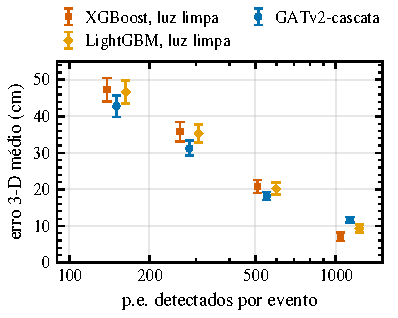
\includegraphics{figures/erro_luz.pdf}
    \caption{Erro 3-D médio do GATv2\discretionary{-}{-}{-}cascata e, na luz limpa, do \mbox{XGBoost} e do \mbox{LightGBM}, por quartil da luz detectada nos \num{937} eventos de teste; pontos na luz média do quartil, os dos \textit{boosters} deslocados para os lados, e barras de \qty{95}{\percent} de cada média, por \textit{boot\-strap} sobre os eventos do quartil. O GATv2\discretionary{-}{-}{-}cascata erra menos nos três mais escuros, e o \mbox{XGBoost}, no mais claro (\qty{773}{\pe} ou mais); o intervalo da diferença pareada entre os dois exclui o zero em todos os quartis.}
    \label{fig:erro_luz}
  \end{subfigure}\hfill
  \begin{subfigure}[t]{0.485\textwidth}
    \centering
    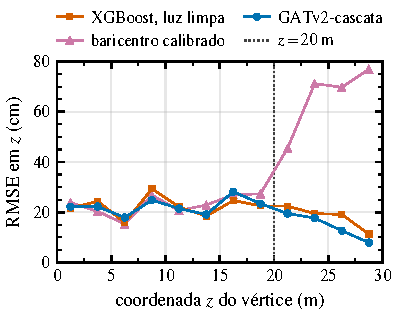
\includegraphics{figures/erro_z.pdf}
    \caption{RMSE em $z$ do GATv2-cascata, do baricentro calibrado e do \mbox{XGBoost} na luz limpa nos eventos de teste, por faixa de \qty{2.5}{\m} do $z$ do vértice; linha pontilhada em \qty{20}{\m}. Até \qty{20}{\m}, os erros são próximos; perto da tampa ($z = {}$\qty{29.93}{\m}), o do baricentro sobe e o do GATv2-cascata cai.}
    \label{fig:erro_z}
  \end{subfigure}
  \caption{Onde o erro se concentra nos eventos de teste: (a)~por quartil de luz detectada; (b)~por faixa de $z$ do vértice.}
  \label{fig:par_onde_erro}
\end{figure}

\subsection{O que limita a resolução}
\label{sec:limites}

No sorteio nominal do teste, o RMSE em $z$ do baricentro calibrado cai de \num{55.18} para \qty{37.02}{\cm} entre as eficiências $\varepsilon$ de \num{0.005} e \num{1}, e de \num{42.45} para \qty{35.24}{\cm} entre as energias de \num{10} e \qty{100}{\MeV} (a Figura~\ref{fig:baricentro_luz} mostra médias). Com \qty{177.8}{\pe\per\MeV} em média, perto do rendimento médio do APEX, fica em \qty{38.23}{\cm} e, abaixo de $z = {}$\qty{20}{\m}, com menos luz, em \qty{13.79}{\cm}, próximo dos \qty{13.7}{\cm} do APEX a \qty{10}{\MeV} (Tabela~\ref{tab:referencias}). Detectar todos os fótons reduziria o erro do baricentro em \qty{5.43}{\cm} (\qty{4.96}{\cm} na média dos sorteios), e mais ainda sem o arredondamento da Equação~\eqref{eq:luz}, que a \qty{10}{\MeV} zera os canais mais fracos e eleva esse erro; por isso, com a mesma luz detectada, a varredura em energia fica abaixo da varredura em eficiência. No conjunto do teste, o erro do baricentro é sobretudo sistemático: com $\varepsilon = {}$\num{0.02}, o GATv2\discretionary{-}{-}{-}cascata (\qty{20.46}{\cm}) já erra menos em $z$ que o baricentro com todos os fótons. Essa parte sistemática vem dos vértices a partir de \qty{20}{\m}, onde o baricentro fica em \qty{63.16}{\cm} mesmo com todos os fótons (Seção~\ref{sec:onde_erro}); abaixo de \qty{20}{\m}, seu erro é sobretudo estatístico: de \qty{23.29}{\cm}, perto dos \qty{22.54}{\cm} do GATv2\discretionary{-}{-}{-}cascata, cai para \qty{8.33}{\cm} com todos os fótons.

O erro do GATv2-cascata também cai com mais luz (Seção~\ref{sec:onde_erro}), mas a luz diminui longe das paredes longas, e os modelos só foram treinados com \qty{10}{\MeV} e $\varepsilon = {}$\num{0.02}: para eles, nenhuma varredura separa o efeito da estatística de fótons do da posição. A influência da cobertura da grade não foi isolada. Com o treino completo, todo vértice de teste tem um de treino a no máximo \qty{50}{\cm}; com um quarto dos eventos, como na primeira comparação (Seção~\ref{sec:dificuldades}), \qty{27.6}{\percent} dos vértices de teste ficam sem esse vizinho, e a distância média sobe de \num{49.31} para \qty{56.18}{\cm}. Os modelos leem ainda \num{33} escalares do evento construídos à mão, e, na configuração final, nenhum experimento separou deles a contribuição da passagem de mensagens: o resultado é dos codificadores em grafos com esses escalares, não da passagem de mensagens nem da representação em grafos isoladamente.

\subsection{Dificuldades Encontradas}
\label{sec:dificuldades}

Os dados tinham dois defeitos de geometria, um escondido pelo outro: vértices e canais em referenciais diferentes; tampas giradas em torno de $x$, com $y$ e $z$ invertidos. Ambos foram identificados pelo padrão da luz, e os modelos existentes, retreinados. Mudanças de formato sem retrocompatibilidade inutilizaram os pontos de verificação antigos, e nenhuma execução anterior a 4 de agosto de 2026 permanece.

Na primeira comparação, em 4 de agosto de 2026, os codificadores usaram um quarto dos eventos de treino (\num{1872}), sem espelhamento, e \num{9} escalares do evento; o menor MAE médio de teste foi de \qty{18.05}{\cm}, contra \qty{13.01}{\cm} do XGBoost, ambos em luz com aumento. Um diagnóstico registrado durante o projeto, não reproduzido neste relatório, atribuiu cerca de \qty{1.9}{\cm} da diferença ao tamanho do treino, \qty{1.9}{\cm} aos atributos agregados ausentes, \qty{1.0}{\cm} à busca de hiperparâmetros e ao espelhamento dos \textit{boosters}, e \qty{0.3}{\cm} ao restante, a contribuição conjunta de nós, arestas e passagem de mensagens. Medido nos eventos de teste da comparação final, ele levou ao treino completo, aos \num{33} escalares e à avaliação logo após cada treino. A comparação final mudou esses e outros ajustes de uma vez e usou luz limpa; nela, o menor MAE médio foi de \qty{12.63}{\cm}.

A GPU local tinha \qty{3.63}{\gibi\byte}: nos modelos com atenção global, grafos com os \num{6912} canais só cabiam em lotes muito pequenos, daí a restrição aos canais ativos; na primeira comparação, GCN, TransformerConv e GPS-lite falharam por falta de memória. A comparação final, em outra GPU, de \qty{23.98}{\gibi\byte}, parou sem mensagem de erro após treinar \num{11} dos \num{14} codificadores; faltaram os mesmos três.

Os \textit{boosters} foram avaliados em luz com aumento de dados, com luz média do teste \qty{4.1}{\percent} menor que a limpa; reavaliado na luz limpa neste relatório, o XGBoost tem MAE médio \qty{0.20}{\cm} maior (Seções~\ref{sec:protocolo_comparacao} e~\ref{sec:comparacao_referencias}).

\subsection{Alterações no Projeto}
\label{sec:alteracoes}

Em relação ao plano inicial, a representação passou de \num{60} descritores com uma rede densa para grafos dos canais ativos, porque os descritores resumem a leitura do detector inteiro; os modelos finais, porém, ainda leem \num{33} escalares do evento construídos à mão. Em vez de uma só arquitetura, foram comparados \num{11} codificadores de capacidade equiparada, para que o número de parâmetros não decidisse o resultado. \textit{Boosters} ajustados a atributos agregados entraram como referência depois que, em julho de 2026, um modelo simples de \textit{gradient boosting} superou a GNN da época. A avaliação mudou de uma partição de \qty{80}{\percent} e \qty{20}{\percent}, com validação cruzada em \num{10} partes, para uma divisão estratificada fixa de \num{7490}, \num{937} e \num{937} eventos, comum a todos os modelos; a comparação final não teve validação cruzada. O APEX foi comparado em energia igual e também em luz detectada igual, porque sua simulação tem rendimento luminoso médio de \qty{180}{\pe\per\MeV}, \num{3.4} vezes os \num{53.0} do teste.

A extensão a outras energias e geometrias, prevista no plano, não foi feita com os modelos finais; restou a varredura de eficiência e de energia do baricentro (Seção~\ref{sec:limites}). Na comparação final, os codificadores foram treinados sem a busca de hiperparâmetros do plano (Seção~\ref{sec:modelos}), aplicada só aos \textit{boosters} (Seção~\ref{sec:protocolo_comparacao}). Das métricas previstas por eixo, ficaram o RMSE, a média dos três MAE e o $R^2$ só em $z$ (Seção~\ref{sec:onde_erro}); a ordenação e a perda do treinamento usam o erro 3-D médio (Seção~\ref{sec:tarefa}). A comparação com o APEX, proposta por coordenada, ficou restrita a $z$ e à largura combinada, porque a correspondência das larguras transversais com $x$ e $y$ não está estabelecida (Seção~\ref{sec:protocolo_comparacao}). O uso em aquisição em tempo real, esperado no plano, não foi avaliado: o tempo de inferência não foi medido, e os codificadores, com capacidade equiparada a \num{1843395} parâmetros, são maiores que a rede da etapa anterior, de \num{8195}. Essa rede é citada, não reavaliada, porque usou outra partição e a geometria anterior às correções e porque o modelo treinado não está disponível.



% ========== CONCLUSÕES ==========
\section{Conclusões}

\label{sec:conclusoes}

Os codificadores de passagem de mensagens sobre o grafo dos canais ativos, com os escalares do evento, reconstroem o vértice de depósitos de \qty{10}{\MeV} (média de \qty{530.1}{\pe} por evento de teste) com erro 3-D médio de \num{25.95} a \qty{26.27}{\cm} e RMSE combinado de \num{18.55} a \qty{18.80}{\cm} nos quatro melhores. Com capacidade equiparada, o erro 3-D médio dos \num{11} codificadores varia em até \qty{2.89}{\cm}, e esses quatro não se distinguem nos \num{937} eventos de teste. O GATv2-cascata, escolhido pelo menor erro 3-D médio de teste, tem RMSE por eixo, no referencial dos sensores, de \num{20.45}, \num{14.35} e \qty{20.46}{\cm} em $x$, $y$ e $z$.

Nos mesmos eventos e na luz limpa, o GATv2-cascata tem erro 3-D médio \qty{1.71}{\cm} menor que o do XGBoost e RMSE combinado \qty{2.30}{\cm} menor; é melhor nos eventos escuros e na cauda, mas pior no quartil mais claro. Em $z$, o baricentro calibrado tem RMSE \num{2.07} vezes o do GATv2-cascata por causa dos vértices perto da tampa, onde o erro do baricentro é sistemático, viés que o APEX não encontrou na sua simulação. Abaixo de $z = {}$\qty{20}{\m}, o baricentro fica próximo do GATv2-cascata (\num{23.29} e \qty{22.54}{\cm}), e seu erro é sobretudo estatístico: com todos os fótons, cai para \qty{8.33}{\cm}. O~RMSE combinado do GATv2-cascata é \qty{10.6}{\percent} menor que o da rede da etapa anterior, calculado a partir dos valores publicados por eixo, de outra partição e da geometria anterior às correções; a diferença está em $x$ e $y$, pois em $z$ o valor daquela rede, \qty{20.87}{\cm}, fica dentro do intervalo de \qty{95}{\percent} do GATv2-cascata. Em luz detectada igual com o rendimento médio, esse RMSE combinado é \qty{51.0}{\percent} menor que a largura combinada do APEX (\qty{41.3}{\percent} com o mínimo e \qty{28.0}{\percent} em energia igual), média quadrática de larguras sem definição publicada, lidas de um gráfico de outra simulação. Em~$z$, contra \qty{20.46}{\cm} do GATv2-cascata, o APEX tem \qty{24.8}{\cm} com o rendimento médio, acima do intervalo de \qty{95}{\percent}, e \qty{19.4}{\cm} com o mínimo, dentro dele; só em energia igual, em que detecta \num{3.4} vezes mais luz, é melhor (\qty{13.7}{\cm}).

{\clubpenalty=10000 O erro do GATv2-cascata concentra-se nos eventos escuros, longe das paredes longas (\qty{42.79}{\cm} de erro 3-D médio no quartil mais escuro, contra \qty{11.67}{\cm} no mais claro), mas não se separou o efeito da estatística de fótons do da posição. Os resultados valem para uma energia, uma eficiência, uma geometria, um sorteio de fótons por evento e vértices na grade do treino. Cada codificador foi treinado uma vez, sem a busca de hiperparâmetros feita nos \textit{boosters}, com lotes e passos diferentes; não houve ablação dos \num{33} escalares; os \textit{boosters} foram treinados em luz com aumento; e os eventos de teste já tinham orientado o desenho final dos codificadores.\par}

{\clubpenalty=10000 Como trabalhos futuros, propõe-se treinar e avaliar os codificadores em várias eficiências, energias e geometrias; gerar vários sorteios de fótons por evento e vértices fora da grade; repetir a comparação com orçamento de otimização fixo, busca de hiperparâmetros por codificador, \textit{boosters} ajustados e treinados na luz limpa e várias sementes, com e sem os escalares, em eventos de teste novos; prever as coordenadas a partir dos estados dos canais, para testar se resumir o grafo num só vetor limita a precisão; combinar \textit{boosters} e codificadores, que erram menos em faixas de luz diferentes; comparar com o APEX numa simulação equivalente, confirmando a correspondência dos eixos e a definição da largura; e medir o tempo de inferência por evento.\par}


% ========== AGRADECIMENTOS ==========
\phantomsection
\section*{Agradecimentos}
\addcontentsline{toc}{section}{Agradecimentos}

\label{sec:agradecimentos}

Agradeço ao CNPq pela concessão da bolsa de iniciação científica através do Programa PIBIC-ITA.

Agradeço ao meu orientador, \nomeorientador, pela orientação e pelo apoio durante o desenvolvimento desta pesquisa.


% ========== BIBLIOGRAFIA ==========
\newpage
\phantomsection
\addcontentsline{toc}{section}{\refname}
\bibliography{referencias}

\end{document}
